%%
%% getstart.tex -- Flight Gear documentation: Installation and Getting Started
%% Chapter file
%%
%% Written by Michael Basler, started September 1998.
%%
%% Copyright (C) 2002 Michael Basler (pmb@epost.de)
%%
%%
%% This program is free software; you can redistribute it and/or
%% modify it under the terms of the GNU General Public License as
%% published by the Free Software Foundation; either version 2 of the
%% License, or (at your option) any later version.
%%
%% This program is distributed in the hope that it will be useful, but
%% WITHOUT ANY WARRANTY; without even the implied warranty of
%% MERCHANTABILITY or FITNESS FOR A PARTICULAR PURPOSE.  See the GNU
%% General Public License for more details.
%%
%% You should have received a copy of the GNU General Public License
%% along with this program; if not, write to the Free Software
%% Foundation, Inc., 675 Mass Ave, Cambridge, MA 02139, USA.
%%
%% $Id: flight.tex,v 0.5 2002/15/02 michael
%% (Log is kept at end of this file)

%%%%%%%%%%%%%%%%%%%%%%%%%%%%%%%%%%%%%%%%%%%%%%%%%%%%%%%%%%%%%%%%%%%%%%%%%%%%%%%%%%%%%%%%%%%%%%%%%
\chapter{In-flight: All about instruments, keystrokes and menus\label{flight}}
%%%%%%%%%%%%%%%%%%%%%%%%%%%%%%%%%%%%%%%%%%%%%%%%%%%%%%%%%%%%%%%%%%%%%%%%%%%%%%%%%%%%%%%%%%%%%%%%%
\markboth{\thechapter.\hspace*{1mm} FLIGHT}{\thesection\hspace*{1mm} KEYBOARD CONTROLS}

The following is a description of the main systems for controlling the
program and piloting the plane: Historically, \Index{keyboard controls} were developed
first, and you can still control most of the simulator via the keyboard alone. Later on,
they were supplemented by several menu entries, making the interface more accessible,
particularly for beginners, and providing additional functionality. 

For getting a real feeling of flight, you should definitely consider getting a \Index{joystick} or -- preferred -- a \Index{yoke} plus \Index{rudder pedals}. In any case, you
can specify your device of choice for control via the \texttt{-$ $-control-mode} option,
i.e. select joystick, \Index{keyboard}, \Index{mouse}. The default setting is joystick.
Concerning instruments, there are again two alternatives: You can use the panel or the
HUD.

A short leaflet based on this chapter can be found at
 \medskip

\web{http://www.flightgear.org/Docs/InstallGuide/FGShortRef.html}.
 \medskip

\noindent
A version of this leaflet can also be opened via \FlightGear{}'s help menu.

%%%%%%%%%%%%%%%%%%%%%%%%%%%%%%%%%%%%%%%%%%%%%%%%%%%%%%%%%%%%%%%%%%%%%%%%%%%%%%%%%%%%%%%%%%%%%%%%%
\section{Starting the engine}\index{engine!starting}
%%%%%%%%%%%%%%%%%%%%%%%%%%%%%%%%%%%%%%%%%%%%%%%%%%%%%%%%%%%%%%%%%%%%%%%%%%%%%%%%%%%%%%%%%%%%%%%%%

Depending on your situation, when you start the simulator the \Index{engine}s may be on or off. When they are on you just can go on with the start. When they are off, you have to start them first. The \Index{ignition switch} for starting the engine is situated in the lower left corner of the panel. It is shown in Fig.\,4.
\medskip

 \centerline{\fbox{
\includegraphics[clip,width=12.5cm]{magnet2}
}}

\smallskip
 \noindent
Fig.\,4: \textit{The ignition switch.}
\medskip

It has five positions: ''OFF'', ''L'', ''R'', ''BOTH'', and ''START''.  The extreme right position is for starting the engine. For starting the engine, put it onto the position ''BOTH'' using the mouse first. 

Keep in mind that the \Index{mixture lever} has to be at 100\,\% (all the way in) for starting the engine -- otherwise you will fail. In addition, advance the \Index{throttle} to about 25\,\%.

Operate the \Index{starter} using the SPACE key now. When pressing the SPACE key you will observe the ignition switch to change to the position ''START'' and the engine to start after a few seconds.  Afterwards you can bring the throttle back to idle (all the way out).

In addition, have a look if the \Index{parking brake}s are on (red field lit). If so, press the ''B'' button to release them.

%%%%%%%%%%%%%%%%%%%%%%%%%%%%%%%%%%%%%%%%%%%%%%%%%%%%%%%%%%%%%%%%%%%%%%%%%%%%%%%%%%%%%%%%%%%%%%%%%
\section{Keyboard controls}\index{keyboard controls}
%%%%%%%%%%%%%%%%%%%%%%%%%%%%%%%%%%%%%%%%%%%%%%%%%%%%%%%%%%%%%%%%%%%%%%%%%%%%%%%%%%%%%%%%%%%%%%%%%

While \Index{joystick}s or \Index{yoke}s are supported as are \Index{rudder} pedals, you
can fly \FlightGear{} using the keyboard alone. For proper control of the plane during
flight via the keyboard (i) the \texttt{\Index{NumLock}} key must be switched on (ii) the
\FlightGear{} window must have focus (if not, click with the mouse onto the graphics
window). Several of the keyboard controls might be helpful even in case you use a
joystick or yoke.

After activating \texttt{NumLock} the following main \Index{keyboard controls} for driving the plane should work:
 \eject

\noindent
 Tab.\,1: \textit{Main \Index{keyboard controls} for \FlightGear{} on the numeric keypad with
 activated \texttt{NumLock} key:}.
\medskip

\centerline{%%
%% tab1.tex -- Flight Gear documentation: Installation and Getting Started
%% Keyboard controls table 1/Main controls
%%
%% Written by Michael Basler, started September 1998.
%%
%% Copyright (C) 2002 Michael Basler (pmb@epost.de)
%%
%%
%% This program is free software; you can redistribute it and/or
%% modify it under the terms of the GNU General Public License as
%% published by the Free Software Foundation; either version 2 of the
%% License, or (at your option) any later version.
%%
%% This program is distributed in the hope that it will be useful, but
%% WITHOUT ANY WARRANTY; without even the implied warranty of
%% MERCHANTABILITY or FITNESS FOR A PARTICULAR PURPOSE.  See the GNU
%% General Public License for more details.
%%
%% You should have received a copy of the GNU General Public License
%% along with this program; if not, write to the Free Software
%% Foundation, Inc., 675 Mass Ave, Cambridge, MA 02139, USA.
%%
%% $Id: tab1.tex,v 0.5 2002/15/02 michael
%% (Log is kept at end of this file)
%%%%%%%%%%%%%%%%%%%%%%%%%%%%%%%%%%%%%%%%%%%%%%%%%%%%%%%%%%%%%%%%%%%%%%%%%%%%%%%%%%%%%%%%%%%%%%%%
\begin{tabular}{|l|l|}\hline
   Key    &  Action\\\hline
 Pg Up/Pg Dn               &  Throttle\index{throttle}\\
 Left Arrow/Right Arrow    &  Aileron\index{aileron}\\
 Up Arrow/Down Arrow       &  Elevator\index{elevator trim}\\
 Ins/Enter                 &  Rudder\index{rudder}\\
 5                         &  Center aileron/elevator/rudder\\
 Home/End                  &  Elevator \Index{trim}\\\hline
\end{tabular}

%% revision 0.5 2002/02/15 michael
%% Initial revision}
\vskip5mm

For changing views you have to de-activate \texttt{NumLock}. Now \texttt{Shift} +
$<$\texttt{Numeric Keypad Key}$>$ changes the view as follows:
\medskip

\noindent
 Tab.\,2: \textit{View directions\index{view directions}
accessible after de-activating \texttt{NumLock} on the numeric keypad.}
\medskip

\centerline{%%
%% tab2.tex -- Flight Gear documentation: The FlightGear Manual
%% Keyboard controls table 1/Main controls
%%
%% Written by Michael Basler, started September 1998.
%%
%% Copyright (C) 2002 Michael Basler
%%
%%
%% This program is free software; you can redistribute it and/or
%% modify it under the terms of the GNU General Public License as
%% published by the Free Software Foundation; either version 2 of the
%% License, or (at your option) any later version.
%%
%% This program is distributed in the hope that it will be useful, but
%% WITHOUT ANY WARRANTY; without even the implied warranty of
%% MERCHANTABILITY or FITNESS FOR A PARTICULAR PURPOSE.  See the GNU
%% General Public License for more details.
%%
%% You should have received a copy of the GNU General Public License
%% along with this program; if not, write to the Free Software
%% Foundation, Inc., 675 Mass Ave, Cambridge, MA 02139, USA.
%%
%% $Id: tab1.tex,v 0.6 2002/09/09 michael
%% (Log is kept at end of this file)
%%%%%%%%%%%%%%%%%%%%%%%%%%%%%%%%%%%%%%%%%%%%%%%%%%%%%%%%%%%%%%%%%%%%%%%%%%%%%%%%%%%%%%%%%%%%%%%%
\begin{tabular}{|l|l|}\hline
\IfLanguageName{english}{
  Key      &  Action\\\hline
 9 / 3     &  Throttle\index{throttle}\\
 4 / 6     &  Aileron\index{aileron}\\
 8 / 2     &  Elevator\index{elevator}\\
 0 / Enter &  Rudder\index{rudder}\\
 5         &  Center aileron/elevator/rudder\\
 7 / 1     &  Elevator \Index{trim}\\\hline
}{}
\IfLanguageName{french}{
  Touche      &  Action\\\hline
 9 / 3     &  Commande des gaz\index{gaz}\\
 4 / 6     &  Aileron\index{aileron}\\
 8 / 2     &  Gouverne de profondeur\index{gouverne de profondeur}\\
 0 / Entr\'{e}e &  gouverne de direction\index{gouverne de direction}\\
 5         &  Centrage des ailerons/gouverne de profondeur/direction\\
 7 / 1     &  Trim de la gouverne de profondeur \Index{trim}\\\hline
}{}
\IfLanguageName{italian}{
  Pulsante/i      &  Azione\\\hline
 9 / 3     &  Manetta (Throttle)\index{manetta}\index{throttle}\\
 4 / 6     &  Alettoni\index{Alettoni}\\
 8 / 2     &  Elevatore (timone di coda)\index{Elevatore}\\
 0 / Invio &  Timone di direzione\index{gouverne de direction}\\
 5         &  Centra alettoni, timone di coda e di direzione\\
 7 / 1     &  Regola il trim \Index{trim}\\\hline
}{}

\end{tabular}

%% revision 0.5 2002/02/15 michael
%% Initial revision
}
\vskip5mm

Besides, there are several more options for adapting display on screen:
\vfill
\eject

\noindent
 Tab.\,3: \textit{Display options\index{display options}}
\medskip

\centerline{%%
%% tab3.tex -- Flight Gear documentation: The FlightGear Manual
%% Keyboard controls table 2/View directions
%%
%% Written by Michael Basler, started September 1998.
%%
%% Copyright (C) 2002 Michael Basler
%%
%%
%% This program is free software; you can redistribute it and/or
%% modify it under the terms of the GNU General Public License as
%% published by the Free Software Foundation; either version 2 of the
%% License, or (at your option) any later version.
%%
%% This program is distributed in the hope that it will be useful, but
%% WITHOUT ANY WARRANTY; without even the implied warranty of
%% MERCHANTABILITY or FITNESS FOR A PARTICULAR PURPOSE.  See the GNU
%% General Public License for more details.
%%
%% You should have received a copy of the GNU General Public License
%% along with this program; if not, write to the Free Software
%% Foundation, Inc., 675 Mass Ave, Cambridge, MA 02139, USA.
%%
%% $Id: tab2.tex,v 0.6 2002/09/09 michael
%% (Log is kept at end of this file)
%%%%%%%%%%%%%%%%%%%%%%%%%%%%%%%%%%%%%%%%%%%%%%%%%%%%%%%%%%%%%%%%%%%%%%%%%%%%%%%%%%%%%%%%%%%%%%%%
\begin{tabular}{|c|l|}\hline
\iflanguage{english}{
   Numpad Key  &  View direction\index{view directions}\\\hline
    Shift-8  & Forward\\
    Shift-7  & Left/forward\\
    Shift-4  & Left\\
    Shift-1  & Left/back\\
    Shift-2  & Back\\
    Shift-3  & Right/back\\
    Shift-6  & Right\\
    Shift-9  & Right/forward\\\hline
}{}
\iflanguage{french}{
   Touche pav\'{e} num\'{e}rique & Angle de vue\index{angle de vue}\\\hline
    Shift-8  & Vers l'avant\\
    Shift-7  & Avant/Gauche\\
    Shift-4  & Gauche\\
    Shift-1  & Arri\`{e}re/Gauche\\
    Shift-2  & Arri\`{e}re\\
    Shift-3  & Arri\`{e}re/Droit\\
    Shift-6  & Droit\\
    Shift-9  & Avant/Droit\\\hline
}{}
\end{tabular}

%% revision 0.5 2002/02/15 michael
%% Initial revision
}
\vskip5mm

The \Index{autopilot} is controlled via the following keys:
\medskip

\noindent
 Tab.\,4: \textit{Autopilot and related controls.\index{autopilot controls}}
\medskip

\centerline{%%
%% tab4.tex -- Flight Gear documentation: Installation and Getting Started
%% Keyboard controls table 3/Additional view options
%%
%% Written by Michael Basler, started September 1998.
%%
%% Copyright (C) 2002 Michael Basler (pmb@epost.de)
%%
%%
%% This program is free software; you can redistribute it and/or
%% modify it under the terms of the GNU General Public License as
%% published by the Free Software Foundation; either version 2 of the
%% License, or (at your option) any later version.
%%
%% This program is distributed in the hope that it will be useful, but
%% WITHOUT ANY WARRANTY; without even the implied warranty of
%% MERCHANTABILITY or FITNESS FOR A PARTICULAR PURPOSE.  See the GNU
%% General Public License for more details.
%%
%% You should have received a copy of the GNU General Public License
%% along with this program; if not, write to the Free Software
%% Foundation, Inc., 675 Mass Ave, Cambridge, MA 02139, USA.
%%
%% $Id: tab3.tex,v 0.6 2002/09/09 michael
%% (Log is kept at end of this file)
%%%%%%%%%%%%%%%%%%%%%%%%%%%%%%%%%%%%%%%%%%%%%%%%%%%%%%%%%%%%%%%%%%%%%%%%%%%%%%%%%%%%%%%%%%%%%%%%
\begin{tabular}{|l|l|}\hline
 Key              &         Action\\\hline
 P                &    Toggle \Index{instrument panel} on/off \\
 c                &    Toggle3D/2D cockpit
 											 \index{2D cockpit} (if both are available)
 											 \index{3D cockpit}\index{cockpit}\\
 s                &    Cycle panel style full/mini\\
 Shift-F5/F6      &    Shift the panel in y direction\\
 Shift-F7/F8      &    Shift the panel in x direction\\
 Shift-F3					&    Read a panel from a property list\\
 i/I              &    Minimize/maximize HUD              \\
 h/H              &    Change color  of HUD/toggle HUD off\\
                  &    forward/backward      \\   \hline
  x/X             &    Zoom in/out\\
   v              &    Cycle \Index{view modes} (pilot, chase, tower)\\ \hline
   W              &    Toggle \Index{full screen mode} on/off (3dfx only)\\
   z/Z            &    Change \Index{visibility} (fog)  forward/backward \\
   F8             &    Toggle fog on/off\\
   F2			 				& 	 Refresh Scenery tile cache\\
   F4			 				& 	 Force Lighting update\\
   F9             &    Toggle texturing on/off\\
   F10      			&    Toggle menu on/off\\ \hline   
 \end{tabular}

%% revision 0.5 2002/02/15 michael
%% Initial revision}
\medskip

\noindent Ctrl + T is especially interesting as it makes your \Index{Cessna 172} behave
like a cruise missile. Ctrl + U might be handy in case you feel you're just about to
crash. (Shouldn't real planes sport such a key, too?)

In case the \Index{autopilot} is enabled, some of the numeric keypad keys get a special
meaning:

\noindent
 Tab.\,5: \textit{Special action of keys, if autopilot is enabled.\index{autopilot controls}}
\medskip

\centerline{%%
%% tab5.tex -- Flight Gear documentation: Installation and Getting Started
%% Keyboard controls table 4/autopilot controls
%%
%% Written by Michael Basler, started September 1998.
%%
%% Copyright (C) 2002 Michael Basler
%%
%%
%% This program is free software; you can redistribute it and/or
%% modify it under the terms of the GNU General Public License as
%% published by the Free Software Foundation; either version 2 of the
%% License, or (at your option) any later version.
%%
%% This program is distributed in the hope that it will be useful, but
%% WITHOUT ANY WARRANTY; without even the implied warranty of
%% MERCHANTABILITY or FITNESS FOR A PARTICULAR PURPOSE.  See the GNU
%% General Public License for more details.
%%
%% You should have received a copy of the GNU General Public License
%% along with this program; if not, write to the Free Software
%% Foundation, Inc., 675 Mass Ave, Cambridge, MA 02139, USA.
%%
%% $Id: tab4.tex,v 0.6 2002/09/09 michael
%% (Log is kept at end of this file)
%%%%%%%%%%%%%%%%%%%%%%%%%%%%%%%%%%%%%%%%%%%%%%%%%%%%%%%%%%%%%%%%%%%%%%%%%%%%%%%%%%%%%%%%%%%%%%%%
\begin{tabular}{|l|l|}\hline
 Key              &         Action\\\hline
    Ctrl + A      &         Altitude hold\index{altitude hold} toggle on/off\\
    Ctrl + G      &         Follow glide slope 1 toggle on/off\\
    Ctrl + H      &         Heading hold\index{heading hold} toggle on/off\\
    Ctrl + N      &         Follow NAV 1 radial toggle on/off\\
    Ctrl + S      &         Autothrottle\index{autothrottle} toggle on/off\\
    Ctrl + T      &         Terrain follow toggle on/off\\
    Ctrl + U      &         Add 1000 ft. to your altitude (emergency)\\
    Enter		      &         Increase autopilot heading\\
    F6 		    		&         Toggle autopilot target:\\
                  &         current heading/waypoint\\
    F11           &         Autopilot altitude dialog\\
    F12           &         Autopilot heading dialog\\\hline
\end{tabular}

%% revision 0.5 2002/02/15 michael
%% Initial revision}
\medskip

There are several keys for starting and controlling the engine \index{engine controls}:

\noindent
 Tab.\,6: \textit{Engine control keys}
\medskip

\centerline{%%
%% tab6.tex -- Flight Gear documentation: Installation and Getting Started
%% Keyboard controls table 5/key actions for autopilot enabled
%%
%% Written by Michael Basler, started September 1998.
%%
%% Copyright (C) 2002 Michael Basler (pmb@epost.de)
%%
%%
%% This program is free software; you can redistribute it and/or
%% modify it under the terms of the GNU General Public License as
%% published by the Free Software Foundation; either version 2 of the
%% License, or (at your option) any later version.
%%
%% This program is distributed in the hope that it will be useful, but
%% WITHOUT ANY WARRANTY; without even the implied warranty of
%% MERCHANTABILITY or FITNESS FOR A PARTICULAR PURPOSE.  See the GNU
%% General Public License for more details.
%%
%% You should have received a copy of the GNU General Public License
%% along with this program; if not, write to the Free Software
%% Foundation, Inc., 675 Mass Ave, Cambridge, MA 02139, USA.
%%
%% $Id: tab5.tex,v 0.6 2002/09/09 michael
%% (Log is kept at end of this file)
%%%%%%%%%%%%%%%%%%%%%%%%%%%%%%%%%%%%%%%%%%%%%%%%%%%%%%%%%%%%%%%%%%%%%%%%%%%%%%%%%%%%%%%%%%%%%%%%
\begin{tabular}{|l|l|}\hline
 Key           &         Action\\\hline
    8 / 2      &         Altitude adjust\\
    0 / ,      &         Heading adjust\\
    9 / 3      &         Autothrottle adjust \\\hline
 \end{tabular}

%% revision 0.5 2002/02/15 michael
%% Initial revision}
\medskip

Beside these basic keys there are miscelleneous keys for special actions; some of these you'll probably not want to try during your first flight:

\noindent Tab.\,7: \textit{Miscellaneous keyboard controls.\index{keyboard controls! miscellaneous}}
\medskip

\centerline{%%
%% tab7.tex -- Flight Gear documentation: The FlightGear Manual
%% Keyboard controls table 6/Engine related controls
%%
%% Written by Michael Basler, started September 1998.
%%
%% Copyright (C) 2002 Michael Basler
%%
%%
%% This program is free software; you can redistribute it and/or
%% modify it under the terms of the GNU General Public License as
%% published by the Free Software Foundation; either version 2 of the
%% License, or (at your option) any later version.
%%
%% This program is distributed in the hope that it will be useful, but
%% WITHOUT ANY WARRANTY; without even the implied warranty of
%% MERCHANTABILITY or FITNESS FOR A PARTICULAR PURPOSE.  See the GNU
%% General Public License for more details.
%%
%% You should have received a copy of the GNU General Public License
%% along with this program; if not, write to the Free Software
%% Foundation, Inc., 675 Mass Ave, Cambridge, MA 02139, USA.
%%
%% $Id: tab6.tex,v 0.6 2002/09/09 michael
%% (Log is kept at end of this file)
%%%%%%%%%%%%%%%%%%%%%%%%%%%%%%%%%%%%%%%%%%%%%%%%%%%%%%%%%%%%%%%%%%%%%%%%%%%%%%%%%%%%%%%%%%%%%%%%
\begin{tabular}{|l|l|}\hline
  \ifchinese
  按键   &    操作\\\hline
  !     &    选择第一号发动机\\
  @     &    选择第二号发动机\\
  \#    &    选择第三号发动机\\
  \$    &    选择第四号发动机\\
  $\sim$$ &  选择所有发动机\\\hline
  \{    &    减少所选发动机的磁电机档位\\
  \}    &    增加所选发动机的磁电机档位\\
  s     &    为所选的发动机点火启动\\
  M / m &    贫油/富油所选发动机的油气混合比\\
  N / n &    减少/增加所选发动机的螺旋桨转速 \\\hline
  \fi
\iffalse
\IfLanguageName{english}{
Key      &  Action\\ \hline
   !     & Select 1st engine\\
   @	   & Select 2nd engine\\
  \#     & Select 3rd engine\\
  \$     & Select 4th engine\\
  $\sim$ & Select all engines\\\hline
  \{     & Decrease magneto on selected engine\\
  \}     & Increase magneto on selected engine\\
   s     & Fire starter on selected engine(s)\\
  M / m  & Lean/Enrich selected engine mixture\\
  N / n  & Decrease/Increase selected propeller RPM\\\hline
}{}
\fi
\IfLanguageName{french}{
Touche     &  Action\\ \hline
   !     & S\'{e}l\'{e}ctionne le premier moteur\\
   @	 & S\'{e}l\'{e}ctionne le deuxi\`{e}me moteur\\
  \#     & S\'{e}l\'{e}ctionne le troisi\`{e}me moteur\\
  \$     & S\'{e}l\'{e}ctionne le quatri\`{e}me moteur\\
  $\sim$ & S\'{e}l\'{e}ctionne tous les moteurs\\\hline
  \{     & D\'{e}cr\'{e}mente le magn\'{e}to sur le moteur s\'{e}lectionn\'{e}\\
  \}     & Incr\'{e}mente le magn\'{e}to sur le moteur s\'{e}lectionn\'{e}\\
   s     & D\'{e}marrage du/des moteur(s) s\'{e}lectionn\'{e}(s)\\
  M / m  & Appauvrir/Enrichir le m\'{e}lange du moteur s\'{e}lectionn\'{e}\\
  N / n  & Diminue/Augmente le nombre de tours par minute du moteur s\'{e}lectionn\'{e}\\\hline
}{}
\IfLanguageName{italian}{
Pulsante/i &  Azione\\ \hline
   !     & Seleziona il 1\textdegree{} motore\\
   @	   & Seleziona il 2\textdegree{} motore\\
  \#     & Seleziona il 3\textdegree{} motore\\
  \$     & Seleziona il 4\textdegree{} motore\\
  $\sim$ & Seleziona tutti i motori\\\hline
  \{     & Diminuisce la forza dei magneti sui motori selezionati\\
  \}     & Aumenta la forza dei magneti sui motori selezionati\\
   s     & Avvia i(l) motore/i selezionato/i\\
  M / m  & Impoverisce/Arricchisce la miscela del motore selezionato\\
  N / n  & Diminuisce/Aumenta il passo dell'elica del motore selezionato\\\hline
}{}
\end{tabular}

%% revision 0.5 2002/02/15 michael
%% Initial revision
}
\medskip

\noindent
 Note: If you have difficulty processing the \Index{screenshot} \texttt{fgfs-screen.ppm}
on a windows machine, just recall that simply pressing the ''Print'' key copies the
screen to the clipboard, from which you can paste it into any graphics program.

Finally: Starting from \FlightGear{} 0.7.7  these key bindings\index{key
bindings!configuration} are no longer hard coded, but user-adjustable. You can check and change these setting via the file \texttt{keyboard.xml}\index{keyboard.xml} to
be found in the main \FlightGear{} directory. This is a human readable plain ASCII file.
Although it's perhaps not the best idea for beginners to start just with modifying this
file, more advanced users will find it useful to change key bindings according to what
they like (or, perhaps, know from other simulators).

%%%%%%%%%%%%%%%%%%%%%%%%%%%%%%%%%%%%%%%%%%%%%%%%%%%%%%%%%%%%%%%%%%%%%%%%%%%%%%%%%%%%%%%%%%%%%%%%%
\section{Menu entries}\index{menu entries}
%%%%%%%%%%%%%%%%%%%%%%%%%%%%%%%%%%%%%%%%%%%%%%%%%%%%%%%%%%%%%%%%%%%%%%%%%%%%%%%%%%%%%%%%%%%%%%%%%

By default, the menu is disabled after starting the simulator (you don't see a menu in a real plane, do you?). You can turn it on either using the toggle F10 or just by moving the mouse pointer to the top left corner of the display. In casse you want the menu to disappear just hit F10 again or move the mouse to the bottom of the screen.

At present, the menu provides the following functions.

\begin{itemize}
 \item \textbf{File}
 \begin{itemize}
 \item \textbf{Save flight} Saves\index{save flight} the current flight, by default to \texttt{fgfs.sav}.
 \item \textbf{Load flight} Loads\index{load flight} the current flight, by default from \texttt{fgfs.sav}.
 \item \textbf{Reset} Resets\index{reset flight} you to the selected starting position. Comes handy in case you got
lost or something went wrong.
\item \textbf{Hires Snap Shot} Saves a high resolution Screen Shot\index{screenshot} under\\ \texttt{fgfs-screen-XXX.ppm}.
  \item \textbf{Snap Shot} Saves a normal resolution Screen Shot\index{screenshot} under\\ \texttt{fgfs-screen-XXX.ppm}.
  \item \textbf{Exit} Exits\index{exit} the program.
 \end{itemize}

 \item \textbf{View}\index{view}
 \begin{itemize}
 \item \textbf{Toggle Panel} Toggles instrument \Index{panel} on/off.
 \item \textbf{Pilot Offset} Allows setting a different viewpoint (useful for R/C flying).\index{viewpoint}
 \item \textbf{HUD Alpha} Toggles \Index{antialiasing} of HUD lines on/off.
 \item \textbf{Properties} Provies access to numerous properies managed via \FlightGear{}'s \Index{property manager}. This is actually a quite powerful tool allowing to set all the values in the property tree. Obviously, this is a good place to crash the program by entering a ''bad'' value.
 \end{itemize}
 
\item \textbf{Environment}
 \begin{itemize}
 \item \textbf{Goto Airport} Enter the \Index{airport ID}. For details on how to get the IDs
  see Section \ref{aiportid}.
 \end{itemize}

 \item \textbf{Autopilot}\index{autopilot}
 \begin{itemize}
 \item \textbf{Set Heading} Sets \Index{heading} manually.
 \item \textbf{Set Altitude} Sets \Index{altitude} manually.
 \item \textbf{Add Waypoint} Adds \Index{waypoint} to waypoint list.
 \item \textbf{Skip Current Waypoint} Self explaining.
 \item \textbf{Clear Route} Clears current route.
 \item \textbf{Adjust AP Settings} Allows input of several \Index{autopilot} parameters.
 \item \textbf{Toggle HUD format} Toggles figures of latitude/longitude in \Index{HUD}.
 \end{itemize}
 
 \item\textbf{Network}\index{network} (supposes compile option \texttt{-$ $-with-network-olk})
 \begin{itemize}
 \item \textbf{Toggle Display} Toggle \Index{call sign} etc. on/off.
 \item \textbf{Enter Callsign} Enter your \Index{call sign}.
 \item \textbf{Scan for Daemons} Scan for daemons on the net.
 \item \textbf{Register for FGD} Register for \FlightGear{} Daemon.
 \item \textbf{Unregister for FGD} Unregister from \FlightGear{} Daemon.
 \end{itemize}

 \item \textbf{Help}\index{help}
 \begin{itemize}
 \item \textbf{Help} Should bring up this FlightGear Getting Started
 Guide\index{FlightGear Getting Started Guide}. At present not yet fully
 implemented. Under windows this works via a batch file
  \texttt{webrun.bat} under \texttt{/flightgear}. If you intend to use that feature you
  may have to edit \texttt{webrun.bat}. Under UNIX a
comparable shell script might do. 
 \end{itemize}
\end{itemize}

%%%%%%%%%%%%%%%%%%%%%%%%%%%%%%%%%%%%%%%%%%%%%%%%%%%%%%%%%%%%%%%%%%%%%%%%%%%%%%%%%%%%%%%%%%%%%%%%%
\section{The Instrument Panel\index{panel}\index{instrument panel}}
%%%%%%%%%%%%%%%%%%%%%%%%%%%%%%%%%%%%%%%%%%%%%%%%%%%%%%%%%%%%%%%%%%%%%%%%%%%%%%%%%%%%%%%%%%%%%%%%%

The Cessna instrument panel is activated by default when you start \FlightGear{}$\!$, but can be
de-activated by pressing the ''P'' key.  While a complete description of all the
functions of the instrument panel of a Cessna is beyond the scope of this guide, we will
at least try to outline the main \Index{flight instrument}s or \Index{gauge}s.

All panel levers and knobs can be operated with the mouse To change a control, just click with the left/middle mouse button on the corresponding knob/lever. 
\medskip

 \centerline{\fbox{
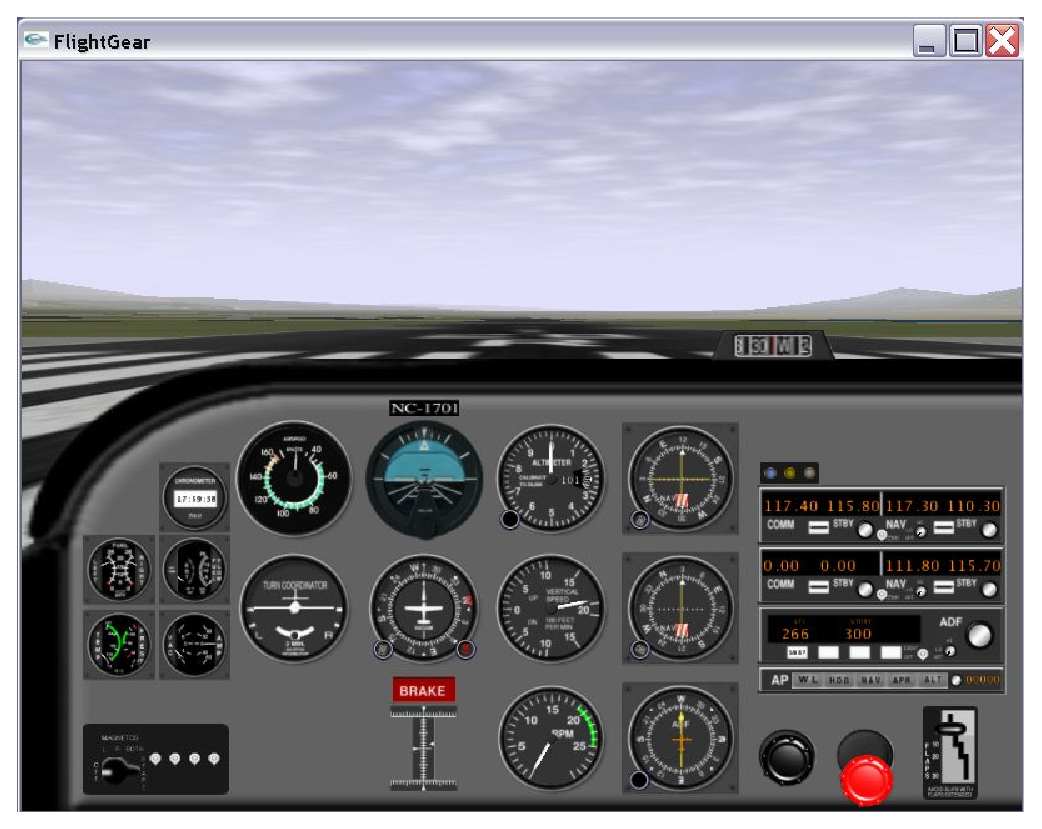
\includegraphics[clip,width=12.5cm]{panel5}
}}

\smallskip
 \noindent
Fig.\,5: \textit{The panel.}
\medskip

Let us start with the most important instruments any simulator pilot must know. In the
center of the instrument panel (Fig.\,5), in the upper row, you will find the
\Index{artificial horizon} (\Index{attitude indicator}) displaying \Index{pitch} and
\Index{bank} of your plane. It has pitch marks as well as bank marks at 10, 20, 30, 60,
and 90 degrees.

Left to the artificial horizon, you'll see the \Index{airspeed indicator}. Not only does
it provide a speed indication in knots but also several arcs showing characteristic
\Index{velocity rages} you have to consider. At first, there is a green arc indicating
the normal operating range of speed with the \Index{flaps} fully retracted. The white arc
indicates the range of speed with flaps in action. The yellow arc shows a range, which
should only be used in smooth air. The upper end of it has a red radial indicating the
speed you must never exceeded - at least as long as you wan't brake your plane.

Below the airspeed indicator you can find the \Index{turn indicator}. The airplane in the
middle indicates the roll of your plane. If the left or right wing of the plane is
aligned with one of the marks, this would indicate a standard turn, i.e. a turn of 360
degrees in exactly two minutes.

Below the plane, still in the turn indicator, is the \Index{inclinometer}. It indicates
if \Index{rudder} and \Index{aileron}s are coordinated. During turns, you always have to
operate \Index{aileron} and \Index{rudder} in such a way that the ball in the tube
remains centered; otherwise the plane is skidding. A simple rule says: ''Step onto the ball'', i.e. step onto the left rudder pedal in case the ball is on the l.h.s.

If you don't have pedals or lack the experience to handle the proper ratio between aileron/rudder automatically, you can start
\FlightGear{} with the option \texttt{-$ $-enable-auto-coordination}.\index{auto
coordination}

To the r.h.s of the artificial horizon you will find the \Index{altimeter} showing the height
above sea level (not ground!) in hundreds of feet.  Below the altimeter is the
\Index{vertical speed indicator} indicating the rate of climbing or sinking of your plane
in hundreds of feet per minute. While you may find it more convenient to use then the
altimeter in cases, keep in mind that its diplay usually has a certain lag in time.

Further below the vertical speed indicator is the RPM (rotations per minute)
indicator\index{RPM indicator}, which displays the rotations per minute  in 100 RPMs. The
green arc marks the optimum region for long-time flight.

The group of the main instruments further includes the \Index{gyro compass} being
situated below the artificial horizon. Besides this one, there is a \Index{magnetic
compass} sitting on top of the panel.

Four of these gauges being arranged in the from of a ''T'' are of special importance: The
air speed indicator, the artificial horizon, the altimeter, and the compass should be
scanned regularly during flight.

Besides these, there are several supplementary instruments. To the very left you will find the
\Index{clock}, obviously being an important tool for instance for determining turn rates.Below the clock there are several smaller gauges displaying the technical state of your engine. Certainly the most important of them is the \Index{fuel indicator} - as any pilot should know.

The \Index{ignition switch} is situated in the lower left corner of the panel (cf. Fig.\,4). It has five positions: ''OFF'', ''L'', ''R'', ''BOTH'', and ''START''. The first one is obvious. ''L'' and ''R'' do not refer to two engines (actually the Cessna does only have one) but to two magnetos being present for safety purposes. The two switch positions can be used for test puposes during preflight. During normal flight the switch should point on ''BOTH''. The extreme right position is for \index{starting the engine} using a battery-powered \Index{starter} (to be operated with the SPACE key in flight gear). 

Like in most flight simulators, you actually get a bit more than in a real plane. The red field directly below the gyro compass displays the state of the \Index{brakes}, i.e., it is lit in case of the brakes being engaged. The instruments below indicate the position of your\Index{yoke}. This serves as kind of a compensation for the missing forces you feel while pushing a real \Index{yoke}. Three of the arrows correspond to the three axes of your yoke/pedal controlling nose up/down, bank left/right, rudder left/right, and throttle. (Keep in mind: They do \textbf{not} reflect the actual position of the plane!) The left vertical arrow indicates elevator trim. 

The right hand side of the panel is occupied by the \Index{radio stack}. Here you find
two \Index{VOR} receivers (NAV),\index{NAV} an \Index{NDB} receiver
(\Index{ADF}) and two \Index{communication radio}s (COMM1/2)\index{COMM1}\index{COMM2} as
well as the autopilot.

The \Index{communication radio} is used for communication with \Index{air traffic
facilities}; it is just a usual radio transceiver working in a special frequency range.
The frequency is displayed in the ''COMM'' field. Usually there are two \Index{COM
transceiver}s; this way you can dial in the frequency of the next controller to contact
while still being in contact with the previous one.

The COM radio can be used to display \Index{ATIS} messages as well. For this purpose, just to dial in the ATIS frequency of the relevant airport.

The \Index{VOR} (Very High Frequency Omni-Directional Range) receiver is used for course
guidance during flight. The frequency of the sender is displayed in the ''\Index{NAV}'' field. In a sense, a VOR acts similarly to a light house permitting to display the position of the
aircraft on a radial around the sender. It transmits one omni-directional ray of radio
waves plus a second ray, the phase of which differs from the first one depending on its
direction (which may be envisaged as kind of a ''rotating'' signal). The phase difference between the two signals allows evaluating the angle of the aircraft on a 360 degrees circle
around the VOR sender, the so-called radial. This radial is then displayed on the gauges
NAV1 and NAV2, resp., left to frequency field. This way it should be clear that the VOR dispaly, while indicating the position of the aircraft relative to the VOR sender, does not say anything about the orientation of the plane. 

Below the two COM/NAV devices is an \Index{NDB} receiver called ADF (automatic direction
finder). Again there is a field displaying the frequency of the facility. The ADF can be
used for navigation, too, but contrary to the VOR does not show the position of the plane
in a radial relative to the sender but the direct heading from the aircraft to the
sender. This is displayed on the gauge below the two NAV gauges.

Above the COMM1 display you will see three LEDs in the colors blue, amber, and white
indicating the outer, middle, and, inner, resp. marker beakon.\index{marker,
outer}\index{marker, inner}\index{marker, middle} These show the distance to the runway
threshold during landing. They to not require the input of a frequency. 

Below the radios you will find the \Index{autopilot}. It has five keys for WL = ''Wing-Leveler'', ''HDG'' = ''Heading'', NAV, APR = ''Glide-Slope'', and ALT = ''Altitude''. These keys when engaged hold the corresponding property. 

A detailed description of the workings of these instruments and their use for navigation
lies beyond this Guide; if you are interested in this exciting topic, we suggest
consulting a book on instrument flight (simulation). Besides, this would be material for
a yet to be written \FlightGear{} Flight School. 

It should be noted, that you can neglect these radio instruments as long as you are strictly flying according to \Index{VFR} (\Index{visual flight rules}). For those wanting to do \Index{IFR} (\Index{instrument flight rules}) flights, it should be mentioned that \FlightGear{} includes a huge database of \Index{navaids} worldwide.

Finally, you find the \Index{throttle}, \Index{mixture}, and flap control\index{flaps} in
the lower right of the panel (recall, flaps can be set via $[$ and $]$ or just using the mouse).

As with the keyboard, the panel\index{panel!reconfiguration} can be re-configured using
configuration files. As these have to be plane specific, they can be found under the
directory of the corresponding plane. As an example, the configuration file for the
default Cessna C172 can be found at \texttt{FlightGear/Aircraft/c172/Panels} as
c172-panel.xml. The accompanying documentation for customizing it (i.e. shifting,
replacing etc. gauges and more) is contained in the file \texttt{README.xmlpanel}\index{README.xmlpanel} written by John Check\index{Check, John},
to be found in the source code in the directory \texttt{docs-mini}.

%%%%%%%%%%%%%%%%%%%%%%%%%%%%%%%%%%%%%%%%%%%%%%%%%%%%%%%%%%%%%%%%%%%%%%%%%%%%%%%%%%%%%%%%%%%%%%%%%
\section{The Head Up Display\index{head up display}}
%%%%%%%%%%%%%%%%%%%%%%%%%%%%%%%%%%%%%%%%%%%%%%%%%%%%%%%%%%%%%%%%%%%%%%%%%%%%%%%%%%%%%%%%%%%%%%%%%

At current, there are two options for reading off the main flight parameters of the
plane: One is the instrument panel already mentioned, while the other one is the
\Index{HUD} (\textbf{H}ead \textbf{U}p \textbf{D}isplay) \index{head up display}. Neither
are \Index{HUD}s used in usual general aviation planes nor in civilian ones. Rather they
belong to the equipment of modern military jets. However, some might find it easier to
fly using the HUD even with general aviation aircraft. Several \Index{Cessna} pilots
might actually love to have one, but technology is simply too expensive for implementing
HUDs in general aviation aircraft. Besides, the HUD displays several useful figures
characterizing simulator performance, not to be read off from the panel.

The \Index{HUD} shown in Fig.\,6  displays all main flight parameters of the plane. In
the center you find the \Index{pitch indicator} (in degrees) with the \Index{aileron
indicator} above and the \Index{rudder indicator} below. A corresponding scale for the
elevation\index{elevation indicator} can be found to the left of the pitch scale. On the
bottom there is a simple \Index{turn indicator}.

There are two scales at the extreme left: The inner one displays the \Index{speed} (in
kts) while the outer one indicates position of the \Index{throttle}. The Cessna 172 takes
off at around 55 kts. The two scales on the extreme r.h.s display your \Index{height},
i.\,e. the left one shows the height above ground while the right of it gives that above
zero, both being displayed in feet.

Besides this, the \Index{HUD} delivers some additions information. On the upper left you
will find date and time. Besides,  \Index{latitude} and \Index{longitude}, resp., of your current position are shown on top.

You can change color of the \textbf{HUD} using the ''H'' or ''h''  key. Pressing ethe toggle ''i/I'' minimizes/maximizes the HUD.

\medskip

 \centerline{\fbox{
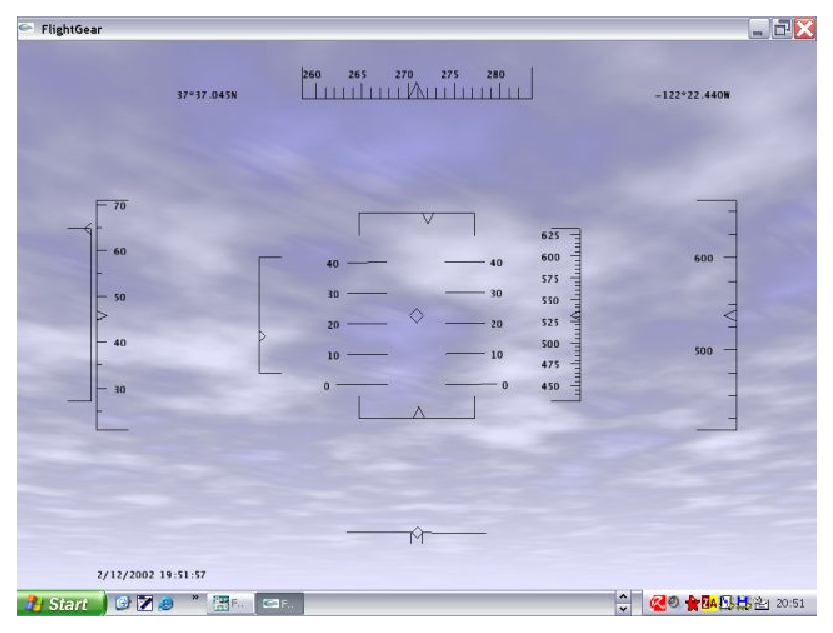
\includegraphics[clip,width=12.5cm]{hud2}
}}

\smallskip
 \noindent
Fig.\,6: \textit{The HUD, or Head Up Display.}
\medskip

%%%%%%%%%%%%%%%%%%%%%%%%%%%%%%%%%%%%%%%%%%%%%%%%%%%%%%%%%%%%%%%%%%%%%%%%%%%%%%%%%%%%%%%%%%%%%%%%%
\section{Mouse controlled actions\index{mouse, actions}}
%%%%%%%%%%%%%%%%%%%%%%%%%%%%%%%%%%%%%%%%%%%%%%%%%%%%%%%%%%%%%%%%%%%%%%%%%%%%%%%%%%%%%%%%%%%%%%%%%

Besides just clicking the menues, your mouse has got certain valuable functions in \FlightGear{}$\!$.


There are three \Index{mouse modi}.\index{mouse} In the normal mode (pointer curser) panel's controls can be operated with the mouse. To change a control, click with the left/middle mouse button on the corresponding knob/lever. While the left mouse button leads to small increments/decrements, the middle one makes greater ones. Clicking on the left hand side of the knob/lever decreases the value, while clicking on the right hand side increases
it.

 Right clicking the mouse activates the simulator control mode (cross hair cursor). This allows control of aileron/elevator via the mouse in absence of a joystick/yoke (enable \texttt{-$ $-enable-auto-coordination} in this case). If you have a joystick you certainly will not make use of this mode

 Right clicking the mouse another time activates the view control mode (arrow cursor).
 This allows changing direction of view, i.e. pan and tilt the view, via the mouse.

 Right clicking the mouse once more resets it into the initial state.

If you are looking for some interesting \Index{places to discover} with \FlightGear{}
(which may or may not require downloading additional scenery) you may want to check
 \medskip

 \web{http://www.flightgear.org/Places/}.
  \medskip

\noindent
 There is now a menu entry for entering directly the \Index{airport code} of the
airport you want to start from.

Finally, if you're done and are about to leave the plane, just hit the ESC key or use the
corresponding menu entry to \Index{exit} the program. It is not suggested to simply
''kill'' the simulator by clicking the text window.

%%%%%%%%%%%%%%%%%%%%%%%%%%%%%%%%%%%%%%%%%%%%%%%%%%%%%%%%%%%%%%%%%%%%%%%%%%%%%%%%%%%%%%%%%%%%%%%%%
\section{Some further reading for pilot students\label{flightschoool}\index{flight schools}\index{text books}}
%%%%%%%%%%%%%%%%%%%%%%%%%%%%%%%%%%%%%%%%%%%%%%%%%%%%%%%%%%%%%%%%%%%%%%%%%%%%%%%%%%%%%%%%%%%%%%%%%

In view of that fact, that there is not yet a \FlightGear{} specific flight course, here
are some useful hints to texts for those who want to learn piloting a plane.

First, a quite comprehensive manual is the \Index{Aeronautical Information Manual},
published by the \Index{FAA}, and being online available at
\medskip

\web{http://www.faa.gov/ATPubs/AIM/}.
\medskip

 \noindent
This is the Official Guide to Basic Flight Information and ATC Procedures by the FAA. It
contains a lot of information on flight rules, flight safety, navigation, and more. If
you find this a bit too hard reading, you may prefer the \Index{FAA Training Book},
\medskip

\web{http://avstop.com/AC/FlightTraingHandbook/},
\medskip

 \noindent
which covers all aspects of flight, beginning with the theory of flight and the working
of airplanes, via procedures like takeoff and landing up to emergency situations. This is
an ideal reading for those who want to learn some basics on flight but don't (yet) want
to spend bucks on getting a costly paper pilot's handbook.

While the handbook mentioned above is an excellent introduction on \Index{VFR} (visual
fligtht rules), it does not include flying according to \Index{IFR} (instrument flight
rules). However, an excellent introduction into navigation and flight according to
Instrument Flight Rules written by Charles Wood\index{Wood, Charles} can be found at

\web{http://www.navfltsm.addr.com/}.

Another comprehensive but yet readable text is John Denker's\index{Denker, John}
''\Index{See how it flies}'', available at
\medskip

\web{http://www.monmouth.com/~jsd/how/htm/title.html}.
\medskip

 \noindent
This is a real online text book, beginning with Bernoulli's principle, drag and power,
and the like, with the later chapters covering even advanced aspects of VFR as well as
IFR flying


%% Revision 0.00  1998/09/08  michael
%% Initial revision for version 0.53.
%% Revision 0.01  1998/09/20  michael
%% several extensions and corrections, added Fig.1.
%% revision 0.10  1998/10/01  michael
%% final proofreading for release
%% revision 0.11  1998/11/01  michael
%% Complete revision of keyborad controls, interesting places
%% revision 0.12  1999/03/07  michael
%% Corrected rudder key
%% revision 0.20  1999/06/04  michael
%% HUD completely rewritten, added panel section with picture, and menu section
%% updated keystrokes
%% revision 0.3 2000/04/20 michael
%% again updated and added keystrokes
%% revised menu entries
%% picture of new panel and re-written panel section
%% added mouse control section
%% Updated many keys, notably autopilot related, added two new tables
%% revision 0.4 2001/05/12 michael
%% updated/added many keystrikes, updated/added panel description
%% (radio stack etc.), new panel pic, panel before HUD now
%% short description of VOR/NDB
%% revision 0.41 2001/01/01 michael
%% added section on flight school material
%% added hints to user configurable *.xml files
%% revision 0.5 2002/01/01 michael
%% revised all changed keybindings now mostly read off of keyboard.xml
%% restructured tables more logically and put into separate files 
%% for inclusion in Short Reference
%% New panel picture and revised descirption of panel according to new features
%% New HUD picture